\batchmode
\documentclass[twoside]{book}

% Packages required by doxygen
\usepackage{fixltx2e}
\usepackage{calc}
\usepackage{doxygen}
\usepackage[export]{adjustbox} % also loads graphicx
\usepackage{graphicx}
\usepackage[utf8]{inputenc}
\usepackage{makeidx}
\usepackage{multicol}
\usepackage{multirow}
\PassOptionsToPackage{warn}{textcomp}
\usepackage{textcomp}
\usepackage[nointegrals]{wasysym}
\usepackage[table]{xcolor}

% Font selection
\usepackage[T1]{fontenc}
\usepackage[scaled=.90]{helvet}
\usepackage{courier}
\usepackage{amssymb}
\usepackage{sectsty}
\renewcommand{\familydefault}{\sfdefault}
\allsectionsfont{%
  \fontseries{bc}\selectfont%
  \color{darkgray}%
}
\renewcommand{\DoxyLabelFont}{%
  \fontseries{bc}\selectfont%
  \color{darkgray}%
}
\newcommand{\+}{\discretionary{\mbox{\scriptsize$\hookleftarrow$}}{}{}}

% Page & text layout
\usepackage{geometry}
\geometry{%
  a4paper,%
  top=2.5cm,%
  bottom=2.5cm,%
  left=2.5cm,%
  right=2.5cm%
}
\tolerance=750
\hfuzz=15pt
\hbadness=750
\setlength{\emergencystretch}{15pt}
\setlength{\parindent}{0cm}
\setlength{\parskip}{3ex plus 2ex minus 2ex}
\makeatletter
\renewcommand{\paragraph}{%
  \@startsection{paragraph}{4}{0ex}{-1.0ex}{1.0ex}{%
    \normalfont\normalsize\bfseries\SS@parafont%
  }%
}
\renewcommand{\subparagraph}{%
  \@startsection{subparagraph}{5}{0ex}{-1.0ex}{1.0ex}{%
    \normalfont\normalsize\bfseries\SS@subparafont%
  }%
}
\makeatother

% Headers & footers
\usepackage{fancyhdr}
\pagestyle{fancyplain}
\fancyhead[LE]{\fancyplain{}{\bfseries\thepage}}
\fancyhead[CE]{\fancyplain{}{}}
\fancyhead[RE]{\fancyplain{}{\bfseries\leftmark}}
\fancyhead[LO]{\fancyplain{}{\bfseries\rightmark}}
\fancyhead[CO]{\fancyplain{}{}}
\fancyhead[RO]{\fancyplain{}{\bfseries\thepage}}
\fancyfoot[LE]{\fancyplain{}{}}
\fancyfoot[CE]{\fancyplain{}{}}
\fancyfoot[RE]{\fancyplain{}{\bfseries\scriptsize Generated by Doxygen }}
\fancyfoot[LO]{\fancyplain{}{\bfseries\scriptsize Generated by Doxygen }}
\fancyfoot[CO]{\fancyplain{}{}}
\fancyfoot[RO]{\fancyplain{}{}}
\renewcommand{\footrulewidth}{0.4pt}
\renewcommand{\chaptermark}[1]{%
  \markboth{#1}{}%
}
\renewcommand{\sectionmark}[1]{%
  \markright{\thesection\ #1}%
}

% Indices & bibliography
\usepackage{natbib}
\usepackage[titles]{tocloft}
\setcounter{tocdepth}{3}
\setcounter{secnumdepth}{5}
\makeindex

% Hyperlinks (required, but should be loaded last)
\usepackage{ifpdf}
\ifpdf
  \usepackage[pdftex,pagebackref=true]{hyperref}
\else
  \usepackage[ps2pdf,pagebackref=true]{hyperref}
\fi
\hypersetup{%
  colorlinks=true,%
  linkcolor=blue,%
  citecolor=blue,%
  unicode%
}

% Custom commands
\newcommand{\clearemptydoublepage}{%
  \newpage{\pagestyle{empty}\cleardoublepage}%
}

\usepackage{caption}
\captionsetup{labelsep=space,justification=centering,font={bf},singlelinecheck=off,skip=4pt,position=top}

%===== C O N T E N T S =====

\begin{document}

% Titlepage & ToC
\hypersetup{pageanchor=false,
             bookmarksnumbered=true
            }
\pagenumbering{alph}
\pagenumbering{arabic}
\hypersetup{pageanchor=true}

%--- Begin generated contents ---
\chapter{Demo problem\+: 2D F\+SI on unstructured meshes with adaptivity}
\label{index}\hypertarget{index}{}\hypertarget{index_q}{}\section{A few quick questions...}\label{index_q}
Since {\ttfamily oomph-\/lib} is developed as open-\/source software, any evidence that the code is being downloaded and used is very helpful for us as it helps to justify our continued work on this project.

We would therefore be extremely grateful if you could provide the information requested in the form below. Pressing the \char`\"{}submit\char`\"{} button will get you to the actual download page.

{\bfseries Note\+:} 
\begin{DoxyItemize}
\item All information will be treated as confidential. 
\item If you provide your email address and check the appropriate box we will add you to our mailing list to inform you of upgrades and bug fixes to the code. Rest assured that the mailing list is {\bfseries very low volume} -- we have better things to do than to bombard you with email. 
\item If you still feel reluctant to provide any of the information requested, feel free to enter some dummy input. The form will check that {\bfseries some} information has been entered but entering your name as \char`\"{}\+Joe Cool\char`\"{} is perfectly acceptable -- this is to discourage people from not providing the information simply because they are too lazy to type... 
\end{DoxyItemize}



 







 

 \hypertarget{index_pdf}{}\section{P\+D\+F file}\label{index_pdf}
A \href{../latex/refman.pdf}{\tt pdf version} of this document is available. \end{document}

\chapter{Namespace Index}
\section{Namespace List}
Here is a list of all namespaces with brief descriptions\+:\begin{DoxyCompactList}
\item\contentsline{section}{\hyperlink{namespaceGlobal__Physical__Variables}{Global\+\_\+\+Physical\+\_\+\+Variables} \\*Global variables that represent physical properties }{\pageref{namespaceGlobal__Physical__Variables}}{}
\item\contentsline{section}{\hyperlink{namespaceoomph}{oomph} }{\pageref{namespaceoomph}}{}
\item\contentsline{section}{\hyperlink{namespacePhysical__Variables}{Physical\+\_\+\+Variables} \\*Namespace for the solution of 2D linear shell equation }{\pageref{namespacePhysical__Variables}}{}
\end{DoxyCompactList}

\chapter{Hierarchical Index}
\section{Class Hierarchy}
This inheritance list is sorted roughly, but not completely, alphabetically\+:\begin{DoxyCompactList}
\item Problem\begin{DoxyCompactList}
\item \contentsline{section}{Unstructured\+Solid\+Problem$<$ E\+L\+E\+M\+E\+NT $>$}{\pageref{classUnstructuredSolidProblem}}{}
\end{DoxyCompactList}
\end{DoxyCompactList}

\chapter{Class Index}
\section{Class List}
Here are the classes, structs, unions and interfaces with brief descriptions\+:\begin{DoxyCompactList}
\item\contentsline{section}{\hyperlink{classPMLProblem}{P\+M\+L\+Problem$<$ E\+L\+E\+M\+E\+N\+T $>$} }{\pageref{classPMLProblem}}{}
\item\contentsline{section}{\hyperlink{classGlobalParameters_1_1TestPMLMapping}{Global\+Parameters\+::\+Test\+P\+M\+L\+Mapping} }{\pageref{classGlobalParameters_1_1TestPMLMapping}}{}
\end{DoxyCompactList}

\chapter{File Index}
\section{File List}
Here is a list of all files with brief descriptions\+:\begin{DoxyCompactList}
\item\contentsline{section}{\hyperlink{jeffery__orbit_8cc}{jeffery\+\_\+orbit.\+cc} }{\pageref{jeffery__orbit_8cc}}{}
\item\contentsline{section}{\hyperlink{jeffery__orbit_8txt__doxygenified_8h}{jeffery\+\_\+orbit.\+txt\+\_\+doxygenified.\+h} }{\pageref{jeffery__orbit_8txt__doxygenified_8h}}{}
\item\contentsline{section}{\hyperlink{my__taylor__hood__elements_8h}{my\+\_\+taylor\+\_\+hood\+\_\+elements.\+h} }{\pageref{my__taylor__hood__elements_8h}}{}
\end{DoxyCompactList}

\chapter{Namespace Documentation}
\hypertarget{namespaceGlobal__Physical__Variables}{}\section{Global\+\_\+\+Physical\+\_\+\+Variables Namespace Reference}
\label{namespaceGlobal__Physical__Variables}\index{Global\+\_\+\+Physical\+\_\+\+Variables@{Global\+\_\+\+Physical\+\_\+\+Variables}}


Namespace for physical parameters.  


\subsection*{Functions}
\begin{DoxyCompactItemize}
\item 
Vector$<$ double $>$ \hyperlink{namespaceGlobal__Physical__Variables_afae321364975eb56688ad13abc8ed6b7}{Gravity} (2)
\begin{DoxyCompactList}\small\item\em Gravity vector. \end{DoxyCompactList}\item 
void \hyperlink{namespaceGlobal__Physical__Variables_a87da705b8a46bed337cf5dbdd788b87b}{body\+\_\+force} (const double \&time, const Vector$<$ double $>$ \&x, Vector$<$ double $>$ \&result)
\begin{DoxyCompactList}\small\item\em Functional body force. \end{DoxyCompactList}\item 
void \hyperlink{namespaceGlobal__Physical__Variables_a9780d615ae07c4e00a436ab2973b54e6}{zero\+\_\+body\+\_\+force} (const double \&time, const Vector$<$ double $>$ \&x, Vector$<$ double $>$ \&result)
\begin{DoxyCompactList}\small\item\em Zero functional body force. \end{DoxyCompactList}\end{DoxyCompactItemize}
\subsection*{Variables}
\begin{DoxyCompactItemize}
\item 
double \hyperlink{namespaceGlobal__Physical__Variables_ab814e627d2eb5bc50318879d19ab16b9}{Re} =100
\begin{DoxyCompactList}\small\item\em Reynolds number. \end{DoxyCompactList}\item 
double \hyperlink{namespaceGlobal__Physical__Variables_ab1a845a672b4d74b304639a976dc65c6}{Re\+\_\+inv\+Fr} =100
\begin{DoxyCompactList}\small\item\em Reynolds/\+Froude number. \end{DoxyCompactList}\end{DoxyCompactItemize}


\subsection{Detailed Description}
Namespace for physical parameters. 

\subsection{Function Documentation}
\mbox{\Hypertarget{namespaceGlobal__Physical__Variables_a87da705b8a46bed337cf5dbdd788b87b}\label{namespaceGlobal__Physical__Variables_a87da705b8a46bed337cf5dbdd788b87b}} 
\index{Global\+\_\+\+Physical\+\_\+\+Variables@{Global\+\_\+\+Physical\+\_\+\+Variables}!body\+\_\+force@{body\+\_\+force}}
\index{body\+\_\+force@{body\+\_\+force}!Global\+\_\+\+Physical\+\_\+\+Variables@{Global\+\_\+\+Physical\+\_\+\+Variables}}
\subsubsection{\texorpdfstring{body\+\_\+force()}{body\_force()}}
{\footnotesize\ttfamily void Global\+\_\+\+Physical\+\_\+\+Variables\+::body\+\_\+force (\begin{DoxyParamCaption}\item[{const double \&}]{time,  }\item[{const Vector$<$ double $>$ \&}]{x,  }\item[{Vector$<$ double $>$ \&}]{result }\end{DoxyParamCaption})}



Functional body force. 



Definition at line 62 of file circular\+\_\+driven\+\_\+cavity.\+cc.



References Re\+\_\+inv\+Fr.



Referenced by main().

\mbox{\Hypertarget{namespaceGlobal__Physical__Variables_afae321364975eb56688ad13abc8ed6b7}\label{namespaceGlobal__Physical__Variables_afae321364975eb56688ad13abc8ed6b7}} 
\index{Global\+\_\+\+Physical\+\_\+\+Variables@{Global\+\_\+\+Physical\+\_\+\+Variables}!Gravity@{Gravity}}
\index{Gravity@{Gravity}!Global\+\_\+\+Physical\+\_\+\+Variables@{Global\+\_\+\+Physical\+\_\+\+Variables}}
\subsubsection{\texorpdfstring{Gravity()}{Gravity()}}
{\footnotesize\ttfamily Vector$<$double$>$ Global\+\_\+\+Physical\+\_\+\+Variables\+::\+Gravity (\begin{DoxyParamCaption}\item[{2}]{ }\end{DoxyParamCaption})}



Gravity vector. 



Referenced by main(), and Quarter\+Circle\+Driven\+Cavity\+Problem$<$ E\+L\+E\+M\+E\+N\+T $>$\+::\+Quarter\+Circle\+Driven\+Cavity\+Problem().

\mbox{\Hypertarget{namespaceGlobal__Physical__Variables_a9780d615ae07c4e00a436ab2973b54e6}\label{namespaceGlobal__Physical__Variables_a9780d615ae07c4e00a436ab2973b54e6}} 
\index{Global\+\_\+\+Physical\+\_\+\+Variables@{Global\+\_\+\+Physical\+\_\+\+Variables}!zero\+\_\+body\+\_\+force@{zero\+\_\+body\+\_\+force}}
\index{zero\+\_\+body\+\_\+force@{zero\+\_\+body\+\_\+force}!Global\+\_\+\+Physical\+\_\+\+Variables@{Global\+\_\+\+Physical\+\_\+\+Variables}}
\subsubsection{\texorpdfstring{zero\+\_\+body\+\_\+force()}{zero\_body\_force()}}
{\footnotesize\ttfamily void Global\+\_\+\+Physical\+\_\+\+Variables\+::zero\+\_\+body\+\_\+force (\begin{DoxyParamCaption}\item[{const double \&}]{time,  }\item[{const Vector$<$ double $>$ \&}]{x,  }\item[{Vector$<$ double $>$ \&}]{result }\end{DoxyParamCaption})}



Zero functional body force. 



Definition at line 70 of file circular\+\_\+driven\+\_\+cavity.\+cc.



Referenced by main().



\subsection{Variable Documentation}
\mbox{\Hypertarget{namespaceGlobal__Physical__Variables_ab814e627d2eb5bc50318879d19ab16b9}\label{namespaceGlobal__Physical__Variables_ab814e627d2eb5bc50318879d19ab16b9}} 
\index{Global\+\_\+\+Physical\+\_\+\+Variables@{Global\+\_\+\+Physical\+\_\+\+Variables}!Re@{Re}}
\index{Re@{Re}!Global\+\_\+\+Physical\+\_\+\+Variables@{Global\+\_\+\+Physical\+\_\+\+Variables}}
\subsubsection{\texorpdfstring{Re}{Re}}
{\footnotesize\ttfamily double Global\+\_\+\+Physical\+\_\+\+Variables\+::\+Re =100}



Reynolds number. 



Definition at line 53 of file circular\+\_\+driven\+\_\+cavity.\+cc.



Referenced by Quarter\+Circle\+Driven\+Cavity\+Problem$<$ E\+L\+E\+M\+E\+N\+T $>$\+::\+Quarter\+Circle\+Driven\+Cavity\+Problem().

\mbox{\Hypertarget{namespaceGlobal__Physical__Variables_ab1a845a672b4d74b304639a976dc65c6}\label{namespaceGlobal__Physical__Variables_ab1a845a672b4d74b304639a976dc65c6}} 
\index{Global\+\_\+\+Physical\+\_\+\+Variables@{Global\+\_\+\+Physical\+\_\+\+Variables}!Re\+\_\+inv\+Fr@{Re\+\_\+inv\+Fr}}
\index{Re\+\_\+inv\+Fr@{Re\+\_\+inv\+Fr}!Global\+\_\+\+Physical\+\_\+\+Variables@{Global\+\_\+\+Physical\+\_\+\+Variables}}
\subsubsection{\texorpdfstring{Re\+\_\+inv\+Fr}{Re\_invFr}}
{\footnotesize\ttfamily double Global\+\_\+\+Physical\+\_\+\+Variables\+::\+Re\+\_\+inv\+Fr =100}



Reynolds/\+Froude number. 



Definition at line 56 of file circular\+\_\+driven\+\_\+cavity.\+cc.



Referenced by body\+\_\+force(), and Quarter\+Circle\+Driven\+Cavity\+Problem$<$ E\+L\+E\+M\+E\+N\+T $>$\+::\+Quarter\+Circle\+Driven\+Cavity\+Problem().


\chapter{Class Documentation}
\hypertarget{classUnstructuredFSIProblem}{}\section{Unstructured\+F\+S\+I\+Problem$<$ F\+L\+U\+I\+D\+\_\+\+E\+L\+E\+M\+E\+NT, S\+O\+L\+I\+D\+\_\+\+E\+L\+E\+M\+E\+NT $>$ Class Template Reference}
\label{classUnstructuredFSIProblem}\index{Unstructured\+F\+S\+I\+Problem$<$ F\+L\+U\+I\+D\+\_\+\+E\+L\+E\+M\+E\+N\+T, S\+O\+L\+I\+D\+\_\+\+E\+L\+E\+M\+E\+N\+T $>$@{Unstructured\+F\+S\+I\+Problem$<$ F\+L\+U\+I\+D\+\_\+\+E\+L\+E\+M\+E\+N\+T, S\+O\+L\+I\+D\+\_\+\+E\+L\+E\+M\+E\+N\+T $>$}}


Unstructured F\+SI Problem.  


Inheritance diagram for Unstructured\+F\+S\+I\+Problem$<$ F\+L\+U\+I\+D\+\_\+\+E\+L\+E\+M\+E\+NT, S\+O\+L\+I\+D\+\_\+\+E\+L\+E\+M\+E\+NT $>$\+:\begin{figure}[H]
\begin{center}
\leavevmode
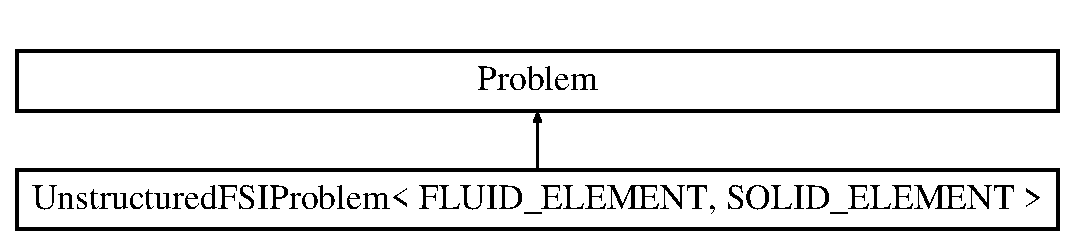
\includegraphics[height=2.000000cm]{classUnstructuredFSIProblem}
\end{center}
\end{figure}
\subsection*{Public Member Functions}
\begin{DoxyCompactItemize}
\item 
\hyperlink{classUnstructuredFSIProblem_a6a31fd839e0215ef1312942cf7284bd2}{Unstructured\+F\+S\+I\+Problem} ()
\begin{DoxyCompactList}\small\item\em Constructor. \end{DoxyCompactList}\item 
\hyperlink{classUnstructuredFSIProblem_a976a81e0dee902f6713bd8ca4d79d000}{$\sim$\+Unstructured\+F\+S\+I\+Problem} ()
\begin{DoxyCompactList}\small\item\em Destructor (empty) \end{DoxyCompactList}\item 
\hyperlink{classFluidTriangleMesh}{Fluid\+Triangle\+Mesh}$<$ F\+L\+U\+I\+D\+\_\+\+E\+L\+E\+M\+E\+NT $>$ $\ast$\& \hyperlink{classUnstructuredFSIProblem_afe86a739cadf57036a0bf351ed9bc1a9}{fluid\+\_\+mesh\+\_\+pt} ()
\begin{DoxyCompactList}\small\item\em Access function for the fluid mesh. \end{DoxyCompactList}\item 
\hyperlink{classMySolidTriangleMesh}{My\+Solid\+Triangle\+Mesh}$<$ S\+O\+L\+I\+D\+\_\+\+E\+L\+E\+M\+E\+NT $>$ $\ast$\& \hyperlink{classUnstructuredFSIProblem_ad1430c627842b8ea0a373adcf571647f}{solid\+\_\+mesh\+\_\+pt} ()
\begin{DoxyCompactList}\small\item\em Access function for the solid mesh. \end{DoxyCompactList}\item 
void \hyperlink{classUnstructuredFSIProblem_a15f581318b505de07f50bd570da8c8d0}{doc\+\_\+solution} (Doc\+Info \&doc\+\_\+info)
\begin{DoxyCompactList}\small\item\em Doc the solution. \end{DoxyCompactList}\end{DoxyCompactItemize}
\subsection*{Private Member Functions}
\begin{DoxyCompactItemize}
\item 
void \hyperlink{classUnstructuredFSIProblem_a934a587c99668fca969a72814b3142a7}{create\+\_\+fsi\+\_\+traction\+\_\+elements} ()
\begin{DoxyCompactList}\small\item\em Create F\+SI traction elements. \end{DoxyCompactList}\item 
void \hyperlink{classUnstructuredFSIProblem_a6f810c300f373cfc79e23d58f95944e3}{create\+\_\+lagrange\+\_\+multiplier\+\_\+elements} ()
\begin{DoxyCompactList}\small\item\em Create elements that enforce prescribed boundary motion for the pseudo-\/solid fluid mesh by Lagrange multipliers. \end{DoxyCompactList}\item 
void \hyperlink{classUnstructuredFSIProblem_a6b86e58ba6cf2871a8e049dd91f6b8b9}{doc\+\_\+solid\+\_\+boundary\+\_\+coordinates} ()
\begin{DoxyCompactList}\small\item\em Sanity check\+: Doc boundary coordinates from solid side. \end{DoxyCompactList}\end{DoxyCompactItemize}
\subsection*{Private Attributes}
\begin{DoxyCompactItemize}
\item 
\hyperlink{classFluidTriangleMesh}{Fluid\+Triangle\+Mesh}$<$ F\+L\+U\+I\+D\+\_\+\+E\+L\+E\+M\+E\+NT $>$ $\ast$ \hyperlink{classUnstructuredFSIProblem_a33c3b4cd9923f8b25368ff20e4810b2c}{Fluid\+\_\+mesh\+\_\+pt}
\begin{DoxyCompactList}\small\item\em Fluid mesh. \end{DoxyCompactList}\item 
\hyperlink{classMySolidTriangleMesh}{My\+Solid\+Triangle\+Mesh}$<$ S\+O\+L\+I\+D\+\_\+\+E\+L\+E\+M\+E\+NT $>$ $\ast$ \hyperlink{classUnstructuredFSIProblem_aeb164665366e237ca311e448466d7c9d}{Solid\+\_\+mesh\+\_\+pt}
\begin{DoxyCompactList}\small\item\em Solid mesh. \end{DoxyCompactList}\item 
Solid\+Mesh $\ast$ \hyperlink{classUnstructuredFSIProblem_ab30c2bc8de791e91d0bba19b048b5219}{Lagrange\+\_\+multiplier\+\_\+mesh\+\_\+pt}
\begin{DoxyCompactList}\small\item\em Pointers to mesh of Lagrange multiplier elements. \end{DoxyCompactList}\item 
Solid\+Mesh $\ast$ \hyperlink{classUnstructuredFSIProblem_ab7ada68f864e990b7b5e40000c289aa1}{Traction\+\_\+mesh\+\_\+pt}
\begin{DoxyCompactList}\small\item\em Vector of pointers to mesh of F\+SI traction elements. \end{DoxyCompactList}\item 
Mesh\+As\+Geom\+Object $\ast$ \hyperlink{classUnstructuredFSIProblem_aa7471e8fb88098faa147e1162480feff}{Solid\+\_\+fsi\+\_\+boundary\+\_\+pt}
\begin{DoxyCompactList}\small\item\em Geom\+Object incarnation of fsi boundary in solid mesh. \end{DoxyCompactList}\end{DoxyCompactItemize}


\subsection{Detailed Description}
\subsubsection*{template$<$class F\+L\+U\+I\+D\+\_\+\+E\+L\+E\+M\+E\+NT, class S\+O\+L\+I\+D\+\_\+\+E\+L\+E\+M\+E\+NT$>$\newline
class Unstructured\+F\+S\+I\+Problem$<$ F\+L\+U\+I\+D\+\_\+\+E\+L\+E\+M\+E\+N\+T, S\+O\+L\+I\+D\+\_\+\+E\+L\+E\+M\+E\+N\+T $>$}

Unstructured F\+SI Problem. 

Definition at line 277 of file unstructured\+\_\+two\+\_\+d\+\_\+fsi.\+cc.



\subsection{Constructor \& Destructor Documentation}
\mbox{\Hypertarget{classUnstructuredFSIProblem_a6a31fd839e0215ef1312942cf7284bd2}\label{classUnstructuredFSIProblem_a6a31fd839e0215ef1312942cf7284bd2}} 
\index{Unstructured\+F\+S\+I\+Problem@{Unstructured\+F\+S\+I\+Problem}!Unstructured\+F\+S\+I\+Problem@{Unstructured\+F\+S\+I\+Problem}}
\index{Unstructured\+F\+S\+I\+Problem@{Unstructured\+F\+S\+I\+Problem}!Unstructured\+F\+S\+I\+Problem@{Unstructured\+F\+S\+I\+Problem}}
\subsubsection{\texorpdfstring{Unstructured\+F\+S\+I\+Problem()}{UnstructuredFSIProblem()}}
{\footnotesize\ttfamily template$<$class F\+L\+U\+I\+D\+\_\+\+E\+L\+E\+M\+E\+NT , class S\+O\+L\+I\+D\+\_\+\+E\+L\+E\+M\+E\+NT $>$ \\
\hyperlink{classUnstructuredFSIProblem}{Unstructured\+F\+S\+I\+Problem}$<$ F\+L\+U\+I\+D\+\_\+\+E\+L\+E\+M\+E\+NT, S\+O\+L\+I\+D\+\_\+\+E\+L\+E\+M\+E\+NT $>$\+::\hyperlink{classUnstructuredFSIProblem}{Unstructured\+F\+S\+I\+Problem} (\begin{DoxyParamCaption}{ }\end{DoxyParamCaption})}



Constructor. 

Constructor for unstructured F\+SI problem. 

Definition at line 339 of file unstructured\+\_\+two\+\_\+d\+\_\+fsi.\+cc.



References Global\+\_\+\+Parameters\+::\+Constitutive\+\_\+law\+\_\+pt, Unstructured\+F\+S\+I\+Problem$<$ F\+L\+U\+I\+D\+\_\+\+E\+L\+E\+M\+E\+N\+T, S\+O\+L\+I\+D\+\_\+\+E\+L\+E\+M\+E\+N\+T $>$\+::doc\+\_\+solid\+\_\+boundary\+\_\+coordinates(), Global\+\_\+\+Parameters\+::gravity(), and Global\+\_\+\+Parameters\+::\+Re.

\mbox{\Hypertarget{classUnstructuredFSIProblem_a976a81e0dee902f6713bd8ca4d79d000}\label{classUnstructuredFSIProblem_a976a81e0dee902f6713bd8ca4d79d000}} 
\index{Unstructured\+F\+S\+I\+Problem@{Unstructured\+F\+S\+I\+Problem}!````~Unstructured\+F\+S\+I\+Problem@{$\sim$\+Unstructured\+F\+S\+I\+Problem}}
\index{````~Unstructured\+F\+S\+I\+Problem@{$\sim$\+Unstructured\+F\+S\+I\+Problem}!Unstructured\+F\+S\+I\+Problem@{Unstructured\+F\+S\+I\+Problem}}
\subsubsection{\texorpdfstring{$\sim$\+Unstructured\+F\+S\+I\+Problem()}{~UnstructuredFSIProblem()}}
{\footnotesize\ttfamily template$<$class F\+L\+U\+I\+D\+\_\+\+E\+L\+E\+M\+E\+NT , class S\+O\+L\+I\+D\+\_\+\+E\+L\+E\+M\+E\+NT $>$ \\
\hyperlink{classUnstructuredFSIProblem}{Unstructured\+F\+S\+I\+Problem}$<$ F\+L\+U\+I\+D\+\_\+\+E\+L\+E\+M\+E\+NT, S\+O\+L\+I\+D\+\_\+\+E\+L\+E\+M\+E\+NT $>$\+::$\sim$\hyperlink{classUnstructuredFSIProblem}{Unstructured\+F\+S\+I\+Problem} (\begin{DoxyParamCaption}{ }\end{DoxyParamCaption})\hspace{0.3cm}{\ttfamily [inline]}}



Destructor (empty) 



Definition at line 286 of file unstructured\+\_\+two\+\_\+d\+\_\+fsi.\+cc.



\subsection{Member Function Documentation}
\mbox{\Hypertarget{classUnstructuredFSIProblem_a934a587c99668fca969a72814b3142a7}\label{classUnstructuredFSIProblem_a934a587c99668fca969a72814b3142a7}} 
\index{Unstructured\+F\+S\+I\+Problem@{Unstructured\+F\+S\+I\+Problem}!create\+\_\+fsi\+\_\+traction\+\_\+elements@{create\+\_\+fsi\+\_\+traction\+\_\+elements}}
\index{create\+\_\+fsi\+\_\+traction\+\_\+elements@{create\+\_\+fsi\+\_\+traction\+\_\+elements}!Unstructured\+F\+S\+I\+Problem@{Unstructured\+F\+S\+I\+Problem}}
\subsubsection{\texorpdfstring{create\+\_\+fsi\+\_\+traction\+\_\+elements()}{create\_fsi\_traction\_elements()}}
{\footnotesize\ttfamily template$<$class F\+L\+U\+I\+D\+\_\+\+E\+L\+E\+M\+E\+NT , class S\+O\+L\+I\+D\+\_\+\+E\+L\+E\+M\+E\+NT $>$ \\
void \hyperlink{classUnstructuredFSIProblem}{Unstructured\+F\+S\+I\+Problem}$<$ F\+L\+U\+I\+D\+\_\+\+E\+L\+E\+M\+E\+NT, S\+O\+L\+I\+D\+\_\+\+E\+L\+E\+M\+E\+NT $>$\+::create\+\_\+fsi\+\_\+traction\+\_\+elements (\begin{DoxyParamCaption}{ }\end{DoxyParamCaption})\hspace{0.3cm}{\ttfamily [private]}}



Create F\+SI traction elements. 



Definition at line 642 of file unstructured\+\_\+two\+\_\+d\+\_\+fsi.\+cc.



References Unstructured\+F\+S\+I\+Problem$<$ F\+L\+U\+I\+D\+\_\+\+E\+L\+E\+M\+E\+N\+T, S\+O\+L\+I\+D\+\_\+\+E\+L\+E\+M\+E\+N\+T $>$\+::create\+\_\+lagrange\+\_\+multiplier\+\_\+elements(), and Global\+\_\+\+Parameters\+::Q.



Referenced by Unstructured\+F\+S\+I\+Problem$<$ F\+L\+U\+I\+D\+\_\+\+E\+L\+E\+M\+E\+N\+T, S\+O\+L\+I\+D\+\_\+\+E\+L\+E\+M\+E\+N\+T $>$\+::doc\+\_\+solid\+\_\+boundary\+\_\+coordinates().

\mbox{\Hypertarget{classUnstructuredFSIProblem_a6f810c300f373cfc79e23d58f95944e3}\label{classUnstructuredFSIProblem_a6f810c300f373cfc79e23d58f95944e3}} 
\index{Unstructured\+F\+S\+I\+Problem@{Unstructured\+F\+S\+I\+Problem}!create\+\_\+lagrange\+\_\+multiplier\+\_\+elements@{create\+\_\+lagrange\+\_\+multiplier\+\_\+elements}}
\index{create\+\_\+lagrange\+\_\+multiplier\+\_\+elements@{create\+\_\+lagrange\+\_\+multiplier\+\_\+elements}!Unstructured\+F\+S\+I\+Problem@{Unstructured\+F\+S\+I\+Problem}}
\subsubsection{\texorpdfstring{create\+\_\+lagrange\+\_\+multiplier\+\_\+elements()}{create\_lagrange\_multiplier\_elements()}}
{\footnotesize\ttfamily template$<$class F\+L\+U\+I\+D\+\_\+\+E\+L\+E\+M\+E\+NT , class S\+O\+L\+I\+D\+\_\+\+E\+L\+E\+M\+E\+NT $>$ \\
void \hyperlink{classUnstructuredFSIProblem}{Unstructured\+F\+S\+I\+Problem}$<$ F\+L\+U\+I\+D\+\_\+\+E\+L\+E\+M\+E\+NT, S\+O\+L\+I\+D\+\_\+\+E\+L\+E\+M\+E\+NT $>$\+::create\+\_\+lagrange\+\_\+multiplier\+\_\+elements (\begin{DoxyParamCaption}{ }\end{DoxyParamCaption})\hspace{0.3cm}{\ttfamily [private]}}



Create elements that enforce prescribed boundary motion for the pseudo-\/solid fluid mesh by Lagrange multipliers. 

Create elements that impose the prescribed boundary displacement for the pseudo-\/solid fluid mesh 

Definition at line 684 of file unstructured\+\_\+two\+\_\+d\+\_\+fsi.\+cc.



References Unstructured\+F\+S\+I\+Problem$<$ F\+L\+U\+I\+D\+\_\+\+E\+L\+E\+M\+E\+N\+T, S\+O\+L\+I\+D\+\_\+\+E\+L\+E\+M\+E\+N\+T $>$\+::doc\+\_\+solution().



Referenced by Unstructured\+F\+S\+I\+Problem$<$ F\+L\+U\+I\+D\+\_\+\+E\+L\+E\+M\+E\+N\+T, S\+O\+L\+I\+D\+\_\+\+E\+L\+E\+M\+E\+N\+T $>$\+::create\+\_\+fsi\+\_\+traction\+\_\+elements().

\mbox{\Hypertarget{classUnstructuredFSIProblem_a6b86e58ba6cf2871a8e049dd91f6b8b9}\label{classUnstructuredFSIProblem_a6b86e58ba6cf2871a8e049dd91f6b8b9}} 
\index{Unstructured\+F\+S\+I\+Problem@{Unstructured\+F\+S\+I\+Problem}!doc\+\_\+solid\+\_\+boundary\+\_\+coordinates@{doc\+\_\+solid\+\_\+boundary\+\_\+coordinates}}
\index{doc\+\_\+solid\+\_\+boundary\+\_\+coordinates@{doc\+\_\+solid\+\_\+boundary\+\_\+coordinates}!Unstructured\+F\+S\+I\+Problem@{Unstructured\+F\+S\+I\+Problem}}
\subsubsection{\texorpdfstring{doc\+\_\+solid\+\_\+boundary\+\_\+coordinates()}{doc\_solid\_boundary\_coordinates()}}
{\footnotesize\ttfamily template$<$class F\+L\+U\+I\+D\+\_\+\+E\+L\+E\+M\+E\+NT , class S\+O\+L\+I\+D\+\_\+\+E\+L\+E\+M\+E\+NT $>$ \\
void \hyperlink{classUnstructuredFSIProblem}{Unstructured\+F\+S\+I\+Problem}$<$ F\+L\+U\+I\+D\+\_\+\+E\+L\+E\+M\+E\+NT, S\+O\+L\+I\+D\+\_\+\+E\+L\+E\+M\+E\+NT $>$\+::doc\+\_\+solid\+\_\+boundary\+\_\+coordinates (\begin{DoxyParamCaption}{ }\end{DoxyParamCaption})\hspace{0.3cm}{\ttfamily [private]}}



Sanity check\+: Doc boundary coordinates from solid side. 

Doc boundary coordinates in solid and plot Geom\+Object representation of F\+SI boundary. 

Definition at line 567 of file unstructured\+\_\+two\+\_\+d\+\_\+fsi.\+cc.



References Unstructured\+F\+S\+I\+Problem$<$ F\+L\+U\+I\+D\+\_\+\+E\+L\+E\+M\+E\+N\+T, S\+O\+L\+I\+D\+\_\+\+E\+L\+E\+M\+E\+N\+T $>$\+::create\+\_\+fsi\+\_\+traction\+\_\+elements().



Referenced by Unstructured\+F\+S\+I\+Problem$<$ F\+L\+U\+I\+D\+\_\+\+E\+L\+E\+M\+E\+N\+T, S\+O\+L\+I\+D\+\_\+\+E\+L\+E\+M\+E\+N\+T $>$\+::\+Unstructured\+F\+S\+I\+Problem().

\mbox{\Hypertarget{classUnstructuredFSIProblem_a15f581318b505de07f50bd570da8c8d0}\label{classUnstructuredFSIProblem_a15f581318b505de07f50bd570da8c8d0}} 
\index{Unstructured\+F\+S\+I\+Problem@{Unstructured\+F\+S\+I\+Problem}!doc\+\_\+solution@{doc\+\_\+solution}}
\index{doc\+\_\+solution@{doc\+\_\+solution}!Unstructured\+F\+S\+I\+Problem@{Unstructured\+F\+S\+I\+Problem}}
\subsubsection{\texorpdfstring{doc\+\_\+solution()}{doc\_solution()}}
{\footnotesize\ttfamily template$<$class F\+L\+U\+I\+D\+\_\+\+E\+L\+E\+M\+E\+NT , class S\+O\+L\+I\+D\+\_\+\+E\+L\+E\+M\+E\+NT $>$ \\
void \hyperlink{classUnstructuredFSIProblem}{Unstructured\+F\+S\+I\+Problem}$<$ F\+L\+U\+I\+D\+\_\+\+E\+L\+E\+M\+E\+NT, S\+O\+L\+I\+D\+\_\+\+E\+L\+E\+M\+E\+NT $>$\+::doc\+\_\+solution (\begin{DoxyParamCaption}\item[{Doc\+Info \&}]{doc\+\_\+info }\end{DoxyParamCaption})}



Doc the solution. 



Definition at line 752 of file unstructured\+\_\+two\+\_\+d\+\_\+fsi.\+cc.



Referenced by Unstructured\+F\+S\+I\+Problem$<$ F\+L\+U\+I\+D\+\_\+\+E\+L\+E\+M\+E\+N\+T, S\+O\+L\+I\+D\+\_\+\+E\+L\+E\+M\+E\+N\+T $>$\+::create\+\_\+lagrange\+\_\+multiplier\+\_\+elements().

\mbox{\Hypertarget{classUnstructuredFSIProblem_afe86a739cadf57036a0bf351ed9bc1a9}\label{classUnstructuredFSIProblem_afe86a739cadf57036a0bf351ed9bc1a9}} 
\index{Unstructured\+F\+S\+I\+Problem@{Unstructured\+F\+S\+I\+Problem}!fluid\+\_\+mesh\+\_\+pt@{fluid\+\_\+mesh\+\_\+pt}}
\index{fluid\+\_\+mesh\+\_\+pt@{fluid\+\_\+mesh\+\_\+pt}!Unstructured\+F\+S\+I\+Problem@{Unstructured\+F\+S\+I\+Problem}}
\subsubsection{\texorpdfstring{fluid\+\_\+mesh\+\_\+pt()}{fluid\_mesh\_pt()}}
{\footnotesize\ttfamily template$<$class F\+L\+U\+I\+D\+\_\+\+E\+L\+E\+M\+E\+NT , class S\+O\+L\+I\+D\+\_\+\+E\+L\+E\+M\+E\+NT $>$ \\
\hyperlink{classFluidTriangleMesh}{Fluid\+Triangle\+Mesh}$<$F\+L\+U\+I\+D\+\_\+\+E\+L\+E\+M\+E\+NT$>$$\ast$\& \hyperlink{classUnstructuredFSIProblem}{Unstructured\+F\+S\+I\+Problem}$<$ F\+L\+U\+I\+D\+\_\+\+E\+L\+E\+M\+E\+NT, S\+O\+L\+I\+D\+\_\+\+E\+L\+E\+M\+E\+NT $>$\+::fluid\+\_\+mesh\+\_\+pt (\begin{DoxyParamCaption}{ }\end{DoxyParamCaption})\hspace{0.3cm}{\ttfamily [inline]}}



Access function for the fluid mesh. 



Definition at line 289 of file unstructured\+\_\+two\+\_\+d\+\_\+fsi.\+cc.



Referenced by main().

\mbox{\Hypertarget{classUnstructuredFSIProblem_ad1430c627842b8ea0a373adcf571647f}\label{classUnstructuredFSIProblem_ad1430c627842b8ea0a373adcf571647f}} 
\index{Unstructured\+F\+S\+I\+Problem@{Unstructured\+F\+S\+I\+Problem}!solid\+\_\+mesh\+\_\+pt@{solid\+\_\+mesh\+\_\+pt}}
\index{solid\+\_\+mesh\+\_\+pt@{solid\+\_\+mesh\+\_\+pt}!Unstructured\+F\+S\+I\+Problem@{Unstructured\+F\+S\+I\+Problem}}
\subsubsection{\texorpdfstring{solid\+\_\+mesh\+\_\+pt()}{solid\_mesh\_pt()}}
{\footnotesize\ttfamily template$<$class F\+L\+U\+I\+D\+\_\+\+E\+L\+E\+M\+E\+NT , class S\+O\+L\+I\+D\+\_\+\+E\+L\+E\+M\+E\+NT $>$ \\
\hyperlink{classMySolidTriangleMesh}{My\+Solid\+Triangle\+Mesh}$<$S\+O\+L\+I\+D\+\_\+\+E\+L\+E\+M\+E\+NT$>$$\ast$\& \hyperlink{classUnstructuredFSIProblem}{Unstructured\+F\+S\+I\+Problem}$<$ F\+L\+U\+I\+D\+\_\+\+E\+L\+E\+M\+E\+NT, S\+O\+L\+I\+D\+\_\+\+E\+L\+E\+M\+E\+NT $>$\+::solid\+\_\+mesh\+\_\+pt (\begin{DoxyParamCaption}{ }\end{DoxyParamCaption})\hspace{0.3cm}{\ttfamily [inline]}}



Access function for the solid mesh. 



Definition at line 295 of file unstructured\+\_\+two\+\_\+d\+\_\+fsi.\+cc.



\subsection{Member Data Documentation}
\mbox{\Hypertarget{classUnstructuredFSIProblem_a33c3b4cd9923f8b25368ff20e4810b2c}\label{classUnstructuredFSIProblem_a33c3b4cd9923f8b25368ff20e4810b2c}} 
\index{Unstructured\+F\+S\+I\+Problem@{Unstructured\+F\+S\+I\+Problem}!Fluid\+\_\+mesh\+\_\+pt@{Fluid\+\_\+mesh\+\_\+pt}}
\index{Fluid\+\_\+mesh\+\_\+pt@{Fluid\+\_\+mesh\+\_\+pt}!Unstructured\+F\+S\+I\+Problem@{Unstructured\+F\+S\+I\+Problem}}
\subsubsection{\texorpdfstring{Fluid\+\_\+mesh\+\_\+pt}{Fluid\_mesh\_pt}}
{\footnotesize\ttfamily template$<$class F\+L\+U\+I\+D\+\_\+\+E\+L\+E\+M\+E\+NT , class S\+O\+L\+I\+D\+\_\+\+E\+L\+E\+M\+E\+NT $>$ \\
\hyperlink{classFluidTriangleMesh}{Fluid\+Triangle\+Mesh}$<$F\+L\+U\+I\+D\+\_\+\+E\+L\+E\+M\+E\+NT$>$$\ast$ \hyperlink{classUnstructuredFSIProblem}{Unstructured\+F\+S\+I\+Problem}$<$ F\+L\+U\+I\+D\+\_\+\+E\+L\+E\+M\+E\+NT, S\+O\+L\+I\+D\+\_\+\+E\+L\+E\+M\+E\+NT $>$\+::Fluid\+\_\+mesh\+\_\+pt\hspace{0.3cm}{\ttfamily [private]}}



Fluid mesh. 



Definition at line 316 of file unstructured\+\_\+two\+\_\+d\+\_\+fsi.\+cc.

\mbox{\Hypertarget{classUnstructuredFSIProblem_ab30c2bc8de791e91d0bba19b048b5219}\label{classUnstructuredFSIProblem_ab30c2bc8de791e91d0bba19b048b5219}} 
\index{Unstructured\+F\+S\+I\+Problem@{Unstructured\+F\+S\+I\+Problem}!Lagrange\+\_\+multiplier\+\_\+mesh\+\_\+pt@{Lagrange\+\_\+multiplier\+\_\+mesh\+\_\+pt}}
\index{Lagrange\+\_\+multiplier\+\_\+mesh\+\_\+pt@{Lagrange\+\_\+multiplier\+\_\+mesh\+\_\+pt}!Unstructured\+F\+S\+I\+Problem@{Unstructured\+F\+S\+I\+Problem}}
\subsubsection{\texorpdfstring{Lagrange\+\_\+multiplier\+\_\+mesh\+\_\+pt}{Lagrange\_multiplier\_mesh\_pt}}
{\footnotesize\ttfamily template$<$class F\+L\+U\+I\+D\+\_\+\+E\+L\+E\+M\+E\+NT , class S\+O\+L\+I\+D\+\_\+\+E\+L\+E\+M\+E\+NT $>$ \\
Solid\+Mesh$\ast$ \hyperlink{classUnstructuredFSIProblem}{Unstructured\+F\+S\+I\+Problem}$<$ F\+L\+U\+I\+D\+\_\+\+E\+L\+E\+M\+E\+NT, S\+O\+L\+I\+D\+\_\+\+E\+L\+E\+M\+E\+NT $>$\+::Lagrange\+\_\+multiplier\+\_\+mesh\+\_\+pt\hspace{0.3cm}{\ttfamily [private]}}



Pointers to mesh of Lagrange multiplier elements. 



Definition at line 322 of file unstructured\+\_\+two\+\_\+d\+\_\+fsi.\+cc.

\mbox{\Hypertarget{classUnstructuredFSIProblem_aa7471e8fb88098faa147e1162480feff}\label{classUnstructuredFSIProblem_aa7471e8fb88098faa147e1162480feff}} 
\index{Unstructured\+F\+S\+I\+Problem@{Unstructured\+F\+S\+I\+Problem}!Solid\+\_\+fsi\+\_\+boundary\+\_\+pt@{Solid\+\_\+fsi\+\_\+boundary\+\_\+pt}}
\index{Solid\+\_\+fsi\+\_\+boundary\+\_\+pt@{Solid\+\_\+fsi\+\_\+boundary\+\_\+pt}!Unstructured\+F\+S\+I\+Problem@{Unstructured\+F\+S\+I\+Problem}}
\subsubsection{\texorpdfstring{Solid\+\_\+fsi\+\_\+boundary\+\_\+pt}{Solid\_fsi\_boundary\_pt}}
{\footnotesize\ttfamily template$<$class F\+L\+U\+I\+D\+\_\+\+E\+L\+E\+M\+E\+NT , class S\+O\+L\+I\+D\+\_\+\+E\+L\+E\+M\+E\+NT $>$ \\
Mesh\+As\+Geom\+Object$\ast$ \hyperlink{classUnstructuredFSIProblem}{Unstructured\+F\+S\+I\+Problem}$<$ F\+L\+U\+I\+D\+\_\+\+E\+L\+E\+M\+E\+NT, S\+O\+L\+I\+D\+\_\+\+E\+L\+E\+M\+E\+NT $>$\+::Solid\+\_\+fsi\+\_\+boundary\+\_\+pt\hspace{0.3cm}{\ttfamily [private]}}



Geom\+Object incarnation of fsi boundary in solid mesh. 



Definition at line 329 of file unstructured\+\_\+two\+\_\+d\+\_\+fsi.\+cc.

\mbox{\Hypertarget{classUnstructuredFSIProblem_aeb164665366e237ca311e448466d7c9d}\label{classUnstructuredFSIProblem_aeb164665366e237ca311e448466d7c9d}} 
\index{Unstructured\+F\+S\+I\+Problem@{Unstructured\+F\+S\+I\+Problem}!Solid\+\_\+mesh\+\_\+pt@{Solid\+\_\+mesh\+\_\+pt}}
\index{Solid\+\_\+mesh\+\_\+pt@{Solid\+\_\+mesh\+\_\+pt}!Unstructured\+F\+S\+I\+Problem@{Unstructured\+F\+S\+I\+Problem}}
\subsubsection{\texorpdfstring{Solid\+\_\+mesh\+\_\+pt}{Solid\_mesh\_pt}}
{\footnotesize\ttfamily template$<$class F\+L\+U\+I\+D\+\_\+\+E\+L\+E\+M\+E\+NT , class S\+O\+L\+I\+D\+\_\+\+E\+L\+E\+M\+E\+NT $>$ \\
\hyperlink{classMySolidTriangleMesh}{My\+Solid\+Triangle\+Mesh}$<$S\+O\+L\+I\+D\+\_\+\+E\+L\+E\+M\+E\+NT$>$$\ast$ \hyperlink{classUnstructuredFSIProblem}{Unstructured\+F\+S\+I\+Problem}$<$ F\+L\+U\+I\+D\+\_\+\+E\+L\+E\+M\+E\+NT, S\+O\+L\+I\+D\+\_\+\+E\+L\+E\+M\+E\+NT $>$\+::Solid\+\_\+mesh\+\_\+pt\hspace{0.3cm}{\ttfamily [private]}}



Solid mesh. 



Definition at line 319 of file unstructured\+\_\+two\+\_\+d\+\_\+fsi.\+cc.

\mbox{\Hypertarget{classUnstructuredFSIProblem_ab7ada68f864e990b7b5e40000c289aa1}\label{classUnstructuredFSIProblem_ab7ada68f864e990b7b5e40000c289aa1}} 
\index{Unstructured\+F\+S\+I\+Problem@{Unstructured\+F\+S\+I\+Problem}!Traction\+\_\+mesh\+\_\+pt@{Traction\+\_\+mesh\+\_\+pt}}
\index{Traction\+\_\+mesh\+\_\+pt@{Traction\+\_\+mesh\+\_\+pt}!Unstructured\+F\+S\+I\+Problem@{Unstructured\+F\+S\+I\+Problem}}
\subsubsection{\texorpdfstring{Traction\+\_\+mesh\+\_\+pt}{Traction\_mesh\_pt}}
{\footnotesize\ttfamily template$<$class F\+L\+U\+I\+D\+\_\+\+E\+L\+E\+M\+E\+NT , class S\+O\+L\+I\+D\+\_\+\+E\+L\+E\+M\+E\+NT $>$ \\
Solid\+Mesh$\ast$ \hyperlink{classUnstructuredFSIProblem}{Unstructured\+F\+S\+I\+Problem}$<$ F\+L\+U\+I\+D\+\_\+\+E\+L\+E\+M\+E\+NT, S\+O\+L\+I\+D\+\_\+\+E\+L\+E\+M\+E\+NT $>$\+::Traction\+\_\+mesh\+\_\+pt\hspace{0.3cm}{\ttfamily [private]}}



Vector of pointers to mesh of F\+SI traction elements. 



Definition at line 325 of file unstructured\+\_\+two\+\_\+d\+\_\+fsi.\+cc.



The documentation for this class was generated from the following file\+:\begin{DoxyCompactItemize}
\item 
\hyperlink{unstructured__two__d__fsi_8cc}{unstructured\+\_\+two\+\_\+d\+\_\+fsi.\+cc}\end{DoxyCompactItemize}

\chapter{File Documentation}
\hypertarget{unstructured__adaptive__2d__fsi_8cc}{}\section{unstructured\+\_\+adaptive\+\_\+2d\+\_\+fsi.\+cc File Reference}
\label{unstructured__adaptive__2d__fsi_8cc}\index{unstructured\+\_\+adaptive\+\_\+2d\+\_\+fsi.\+cc@{unstructured\+\_\+adaptive\+\_\+2d\+\_\+fsi.\+cc}}
\subsection*{Classes}
\begin{DoxyCompactItemize}
\item 
class \hyperlink{classUnstructuredFSIProblem}{Unstructured\+F\+S\+I\+Problem$<$ F\+L\+U\+I\+D\+\_\+\+E\+L\+E\+M\+E\+N\+T, S\+O\+L\+I\+D\+\_\+\+E\+L\+E\+M\+E\+N\+T $>$}
\begin{DoxyCompactList}\small\item\em Unstructured F\+SI problem. \end{DoxyCompactList}\end{DoxyCompactItemize}
\subsection*{Namespaces}
\begin{DoxyCompactItemize}
\item 
 \hyperlink{namespaceGlobal__Physical__Variables}{Global\+\_\+\+Physical\+\_\+\+Variables}
\begin{DoxyCompactList}\small\item\em Global variables. \end{DoxyCompactList}\end{DoxyCompactItemize}
\subsection*{Functions}
\begin{DoxyCompactItemize}
\item 
int \hyperlink{unstructured__adaptive__2d__fsi_8cc_a3c04138a5bfe5d72780bb7e82a18e627}{main} (int argc, char $\ast$$\ast$argv)
\begin{DoxyCompactList}\small\item\em Demonstrate how to solve an unstructured solid problem. \end{DoxyCompactList}\end{DoxyCompactItemize}
\subsection*{Variables}
\begin{DoxyCompactItemize}
\item 
double \hyperlink{namespaceGlobal__Physical__Variables_ab814e627d2eb5bc50318879d19ab16b9}{Global\+\_\+\+Physical\+\_\+\+Variables\+::\+Re} = 0.\+0
\begin{DoxyCompactList}\small\item\em Reynolds number. \end{DoxyCompactList}\item 
double \hyperlink{namespaceGlobal__Physical__Variables_a66cb7ecda9ba0cd72367dd697f154545}{Global\+\_\+\+Physical\+\_\+\+Variables\+::Q} = 0.\+0
\begin{DoxyCompactList}\small\item\em F\+SI parameter. \end{DoxyCompactList}\item 
double \hyperlink{namespaceGlobal__Physical__Variables_a3962c36313826b19f216f6bbbdd6a477}{Global\+\_\+\+Physical\+\_\+\+Variables\+::\+Nu} =0.\+3
\begin{DoxyCompactList}\small\item\em Poisson\textquotesingle{}s ratio. \end{DoxyCompactList}\item 
Constitutive\+Law $\ast$ \hyperlink{namespaceGlobal__Physical__Variables_a2a37fb040c832ee7a086bb13bb02a100}{Global\+\_\+\+Physical\+\_\+\+Variables\+::\+Constitutive\+\_\+law\+\_\+pt} =0
\begin{DoxyCompactList}\small\item\em Pointer to constitutive law. \end{DoxyCompactList}\item 
double \hyperlink{namespaceGlobal__Physical__Variables_a0f1535b448627cbfa0acfb742120d96f}{Global\+\_\+\+Physical\+\_\+\+Variables\+::\+Mesh\+\_\+\+Nu} = 0.\+1
\begin{DoxyCompactList}\small\item\em Mesh poisson ratio. \end{DoxyCompactList}\item 
Constitutive\+Law $\ast$ \hyperlink{namespaceGlobal__Physical__Variables_aac1b52d0b82bc48d24dfcb031d9dc25f}{Global\+\_\+\+Physical\+\_\+\+Variables\+::\+Mesh\+\_\+constitutive\+\_\+law\+\_\+pt} =0
\begin{DoxyCompactList}\small\item\em Pointer to constitutive law for the mesh. \end{DoxyCompactList}\end{DoxyCompactItemize}


\subsection{Function Documentation}
\mbox{\Hypertarget{unstructured__adaptive__2d__fsi_8cc_a3c04138a5bfe5d72780bb7e82a18e627}\label{unstructured__adaptive__2d__fsi_8cc_a3c04138a5bfe5d72780bb7e82a18e627}} 
\index{unstructured\+\_\+adaptive\+\_\+2d\+\_\+fsi.\+cc@{unstructured\+\_\+adaptive\+\_\+2d\+\_\+fsi.\+cc}!main@{main}}
\index{main@{main}!unstructured\+\_\+adaptive\+\_\+2d\+\_\+fsi.\+cc@{unstructured\+\_\+adaptive\+\_\+2d\+\_\+fsi.\+cc}}
\subsubsection{\texorpdfstring{main()}{main()}}
{\footnotesize\ttfamily int main (\begin{DoxyParamCaption}\item[{int}]{argc,  }\item[{char $\ast$$\ast$}]{argv }\end{DoxyParamCaption})}



Demonstrate how to solve an unstructured solid problem. 



Definition at line 926 of file unstructured\+\_\+adaptive\+\_\+2d\+\_\+fsi.\+cc.



References Global\+\_\+\+Physical\+\_\+\+Variables\+::\+Constitutive\+\_\+law\+\_\+pt, Unstructured\+F\+S\+I\+Problem$<$ F\+L\+U\+I\+D\+\_\+\+E\+L\+E\+M\+E\+N\+T, S\+O\+L\+I\+D\+\_\+\+E\+L\+E\+M\+E\+N\+T $>$\+::doc\+\_\+solution(), Global\+\_\+\+Physical\+\_\+\+Variables\+::\+Mesh\+\_\+constitutive\+\_\+law\+\_\+pt, Global\+\_\+\+Physical\+\_\+\+Variables\+::\+Mesh\+\_\+\+Nu, Global\+\_\+\+Physical\+\_\+\+Variables\+::\+Nu, and Global\+\_\+\+Physical\+\_\+\+Variables\+::Q.


\hypertarget{unstructured__adaptive__fsi_8txt__doxygenified_8h}{}\section{unstructured\+\_\+adaptive\+\_\+fsi.\+txt\+\_\+doxygenified.\+h File Reference}
\label{unstructured__adaptive__fsi_8txt__doxygenified_8h}\index{unstructured\+\_\+adaptive\+\_\+fsi.\+txt\+\_\+doxygenified.\+h@{unstructured\+\_\+adaptive\+\_\+fsi.\+txt\+\_\+doxygenified.\+h}}

%--- End generated contents ---

% Index
\backmatter
\newpage
\phantomsection
\clearemptydoublepage
\addcontentsline{toc}{chapter}{Index}
\printindex

